% ============================================================
% TAAI 2026 domestic full-paper track — main file
% 編譯：pdflatex paper_main.tex（跑兩次讓交叉引用/參考文獻正確）
% 依官方範本 taai2026-domestic-full-paper-template-en.pdf 手刻版面
%（該範本無官方 .cls，故用 article class 還原規格）。
% 全英文，pdflatex 可直接編譯。
% ============================================================
\documentclass[10pt]{article}

\usepackage{graphicx}
\usepackage{amsmath, amssymb}
\usepackage{booktabs}
\usepackage{url}
\usepackage{tikz}
\usetikzlibrary{arrows.meta, positioning, shapes.geometric, fit, backgrounds}
\usepackage[T1]{fontenc}
\usepackage{microtype}
\usepackage{times}       % 範本要求 Times-Roman
\usepackage{seqsplit}    % 讓 \texttt 長 identifier（如 superseded_by_iteration）可在窄欄斷行
\usepackage{titlesec}    % 自訂章節標題樣式（全大寫置中編號）
\tolerance=2000\emergencystretch=3em  % 窄欄（83mm）易 overfull，放寬斷字容忍度

% --- TAAI 2026 版面規定（依官方範本 PDF）---
% 印刷區 175mm x 226mm；左邊界 19mm、上邊界 25mm（標題頁除外）；
% 兩欄各 83mm、欄間 8mm；US Letter 紙張（範本未言明紙張，175mm 印刷寬
% 配 19mm 左邊界與 letter 紙寬最吻合，右/下邊界由此還原）。
\usepackage[letterpaper, top=25mm, left=19mm, right=21.9mm, bottom=28.4mm,
            columnsep=8mm]{geometry}
\pagestyle{empty}        % 不設頁碼

% 圖表標題
\usepackage[labelsep=period]{caption}
\captionsetup[figure]{font=small}
\captionsetup[table]{font=small}

% 章節標題：全大寫、置中、加粗，編號後接句點（如 "1. INTRODUCTION"）
\titleformat{\section}{\centering\bfseries\MakeUppercase}{\thesection.}{0.5em}{}
\titleformat{\subsection}{\bfseries}{\thesubsection.}{0.5em}{}
\titleformat{\subsubsection}{\itshape}{\thesubsubsection.}{0.5em}{}
\titlespacing*{\section}{0pt}{*1}{*1}

\begin{document}

\twocolumn[{\centering
\Large\bfseries AN EVALUATION OF MULTI-AGENT LLM SYSTEMS WITH
VERIFICATION-DRIVEN SELF-CORRECTION: A CASE STUDY IN
ACADEMIC LIBRARY ACQUISITION

\vspace{3mm}
\normalsize\mdseries \textsuperscript{1}Ting-Han Wu, \textsuperscript{1,*}Wen-Hung Liao

\vspace{2mm}
\textsuperscript{1}Department of Computer Science, National Chengchi University, Taipei, Taiwan

\textsuperscript{*}E-mail: whliao@nccu.edu.tw

\vspace{5mm}
\par}]

\noindent\textbf{\footnotesize ABSTRACT}\\[1mm]
\footnotesize
Academic library acquisition has long relied on librarians manually
cross-referencing syllabus bibliographies against holdings. This process is hard
to scale, and because it allocates public funds, its outputs face a strong
accountability requirement. A common assumption is that LLMs hallucinate bibliographic
information and thus need external verification. We implement a six-agent LLM
system (with a human-review node) automating the full syllabus-to-acquisition
pipeline, augmented with a Validator$\rightarrow$Discoverer feedback loop for
self-correction. Through four experiments we reach a counterintuitive finding:
under appropriate prompt constraints, LLM hallucination is very low (0--1.4\%),
and the primary bottleneck is verification, not generation: the verifier
mis-pairs records and the queried sources under-cover certain books, neither
stemming from books being nonexistent. A multi-agent architecture thus adds
value not by preventing hallucination but by making every recommendation
auditable and catching detail-level errors.

\vspace{2mm}
\noindent\textbf{Keywords}: AI Agents, Multi-Agent Systems, LLM Evaluation,
Bibliographic Verification, Educational Technology, Accountability
\normalsize
\vspace{3mm}

% ============================================================
\section{Introduction}

Acquisition decisions in academic libraries have long depended on librarians
cross-referencing syllabus readings against current holdings to prioritize
purchases. At our study site, National Chengchi University, over seven thousand
courses are offered in a single semester, their bibliographies scattered across
unstructured text and attachments, inconsistently formatted, titles often
abbreviated or aliased. At this scale, manual cross-referencing is
time-consuming and hard to keep consistent. Automating this process carries
clear educational value, yet it also imposes a requirement distinct from a
general information-extraction task: because acquisition decisions allocate
public
funds, their outputs must be \textit{auditable and traceable}: every purchase
recommendation should be traceable to a verifiable authoritative bibliographic
record, not merely a plausible-looking output. This accountability requirement
is precisely what distinguishes our study, in both design and evaluation, from
work that pursues accuracy alone, placing it at the intersection of agentic AI,
educational technology, and accountability. We scope the system to
textbook-level readings tied to teaching (required and recommended course
texts), not the full breadth of library acquisition such as research monographs,
journals, or special collections.

Facing this task, an intuitive assumption, consistent with the prevailing
consensus in retrieval-augmented generation (RAG) and agentic systems, is that
LLMs are prone to hallucinating bibliographic information, and that the key to
the system therefore lies in introducing an external knowledge base for
verification to prevent errors. On this basis, we design and implement an LLM
pipeline composed of six specialized agents: Crawler, Parser, Discoverer,
Validator, Librarian, and Recommender, plus a human-review node, automating
the entire syllabus-to-acquisition workflow. The system's core
anti-hallucination principle is that all
ISBNs are determined by external authoritative APIs (the National Central
Library NCL/NBINet, the Library of Congress LOC, Google Books, and the Alma
holdings system); the LLM never generates them.

On evaluation, however, this assumption was overturned: hallucination proved
very low (0--1.4\%) while the true bottleneck was the verification stage
(Section IV), over half of the Chinese failures being correctable query defects
rather than nonexistent books. This reframes the architecture's value from
``preventing hallucination'' to ``providing auditability and catching
detail-level errors.''

The contributions of this paper are as follows:

\begin{itemize}
\item \textbf{An architecture-evaluation method for multi-agent LLM systems.}
Using generation-side baselines, namely pure LLM (A) and a single LLM with a
self-invoked tool (B), we quantitatively evaluate correctness and
hallucination, and, via verifier-reliability and failure-cause analyses,
localize our system's bottleneck to verification rather than generation.

\item \textbf{A verification-driven self-correction mechanism, and an honest
account of its limits.} We implement a Validator$\rightarrow$Discoverer
feedback loop that turns the linear pipeline into a self-correcting
collaboration; but we also show that, since generation-side failures are
already rare, its benefit is small and bounded by the structure of failure
causes, itself consistent with our counterintuitive thesis.

\item \textbf{A diagnosis of the verification bottleneck into correctable
defects.} We decompose failure causes into correctable query defects and
coverage gaps requiring source expansion; for the former, our proposed
title-normalization fix recovers 33.0\% of failed Chinese entries directly.
\end{itemize}

The rest of this paper is organized as follows. Section II reviews related work;
Section III describes the data source, system architecture, and evaluation
design; Section IV reports and discusses the results; and Section V concludes.

% ============================================================
\section{Related Work}

\textit{1) Tool-augmented autonomous agents and multi-agent collaboration:}
Recent advances in LLMs have enabled tool-augmented knowledge-discovery
paradigms. The ReAct paradigm lets an LLM interleave reasoning and acting,
decompose complex problems, invoke external tools, and revise intermediate
reasoning based on retrieved evidence~\cite{ReAct}, providing a natural
foundation for multi-step structured tasks. Our Parser, Discoverer, and
Validator agents build on tool-augmented reasoning, with external
bibliographic APIs as their action interface. Standard RAG systems~\cite{RAG}
are designed for semantic-similarity retrieval over unstructured corpora and do
not address the enforced verification of authoritative bibliographies, the
external determination of unique keys such as ISBNs, or the separation of
generation from fact. We adopt a structured multi-agent architecture that
isolates verification as an enforced, dedicated stage. Regarding multi-agent
collaboration, prior work has largely focused on debate- or negotiation-style
reasoning among agents; our collaboration mechanism is instead a
\textit{verification-driven feedback loop}, in which one agent's (the
Validator's) failure signal changes another agent's (the Discoverer's)
behavior, forming a self-correcting closed loop rather than a one-way data
hand-off or a parallel aggregation of opinions.

\textit{2) LLM-based bibliographic extraction and normalization:}
Recent work shows that LLMs can extract structured records from unstructured
scientific text into user-defined schemas~\cite{SIE}, a capability our Parser
builds on for course-syllabus bibliographies. Bibliographic normalization,
however, faces a particular challenge: titles frequently appear as abbreviations,
aliases, traditional--simplified variants, or with volume/subtitle suffixes, so
that exact matching easily fails while loose matching easily mis-pairs to
irrelevant records, especially for short titles. We address this through title
normalization targeting such variants, combined with author matching to avoid
mis-pairing. A non-LLM baseline is instructive here: rule-based extraction is
impractical because syllabus bibliographies are free text with no fixed
schema (Chinese, English, Japanese, and Russian entries in heterogeneous
formats that no finite pattern set captures), and recommendation is generative
by nature, beyond a rule-based method's reach.

\textit{3) Library acquisition and collection decision support:}
Academic library acquisition has traditionally relied on librarians manually
cross-referencing syllabus bibliographies against holdings; prior
decision-support systems have addressed demand-driven collection development in
university digital libraries~\cite{DSS}, but not LLM-based bibliographic
extraction with enforced verification. Our system takes \textit{auditability} as
its design core, anchoring every actionable fact to external authoritative
bibliographic and holdings APIs.

\textit{4) Evaluation methods for LLM systems:}
Evaluating LLMs on factual tasks has motivated metrics beyond exact-match
accuracy: FactScore decomposes long text into atomic facts to measure factual
precision~\cite{FactScore}, RAGAS uses an LLM to verify grounding against
retrieved context~\cite{RAGAS}, and LLM-as-Judge employs a model as an evaluator
of other models' outputs~\cite{LLMJudge}. In contrast, our judgments are grounded
directly against external authoritative records (via API lookup) and validated by
a second human annotator, rather than relying on an LLM judge, which avoids the
same-model self-preference risk in evaluating LLM-generated bibliographies.

% ============================================================
\section{Research Framework}

\subsection{Data Source}
The experiments use the course syllabi of a single semester at National
Chengchi University, comprising 7{,}354 courses. The bibliographic text
(required and recommended readings) of each course is obtained by the Crawler
agent; for courses whose syllabi list no bibliography, the Discoverer agent
recommends references based on the course description. Books extracted by the
Parser and verified by the Validator constitute the population for the
subsequent experiments. The bibliographic text is unstructured, mixes Chinese
and English, and often presents titles as abbreviations, aliases, or with
volume/subtitle variants.

\subsection{System Architecture}

% Fig. 2 —— 系統架構圖（跨欄 figure*，置於 System Architecture 起始）
\begin{figure*}[t]
\centering
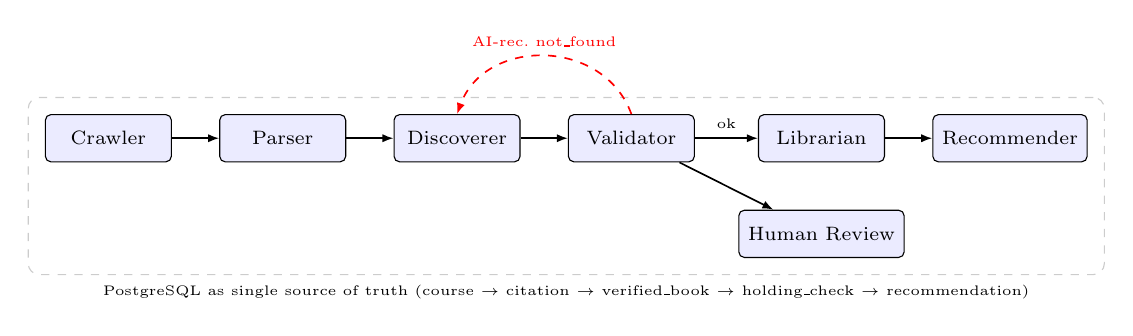
\begin{tikzpicture}[
    font=\footnotesize,
    node distance=4mm and 6mm,
    agent/.style={draw, rounded corners=2pt, minimum height=6mm,
                  minimum width=16mm, align=center, fill=blue!8, font=\scriptsize},
    arr/.style={-{Latex[length=1.4mm]}, semithick},
    loop/.style={-{Latex[length=1.4mm]}, semithick, red, dashed},
]
\node[agent] (crawler) {Crawler};
\node[agent, right=of crawler] (parser) {Parser};
\node[agent, right=of parser] (disc) {Discoverer};
\node[agent, right=of disc] (val) {Validator};
\node[agent, right=8mm of val] (lib) {Librarian};
\node[agent, right=of lib] (rec) {Recommender};
\node[agent, below=6mm of lib] (hr) {Human Review};
\draw[arr] (crawler) -- (parser);
\draw[arr] (parser) -- (disc);
\draw[arr] (disc) -- (val);
\draw[arr] (val) -- node[above, font=\tiny]{ok} (lib);
\draw[arr] (val) -- (hr);
\draw[arr] (lib) -- (rec);
\draw[loop] (val.north) to[out=110, in=70, looseness=1.2]
    node[above, font=\tiny, text=red]{AI-rec.\ not\_found} (disc.north);
\begin{scope}[on background layer]
\node[draw=gray!40, dashed, rounded corners, fit=(crawler)(rec)(hr),
      inner sep=6pt, label={[font=\tiny]below:%
      PostgreSQL as single source of truth
      (course $\to$ citation $\to$ verified\_book $\to$ holding\_check $\to$ recommendation)}]{};
\end{scope}
\end{tikzpicture}
\caption{System architecture. Six specialized agents (plus a human-review node)
form a linear pipeline; a conditional edge (dashed) routes control flow from the
Validator back to the Discoverer when an AI-recommended book fails verification,
forming a verification-driven self-correcting loop.}
\label{fig:arch}
\end{figure*}

The system is built as a directed graph in LangGraph, composed of six
specialized agent nodes, decomposing the ``syllabus $\to$ bibliography $\to$
acquisition recommendation'' flow into stages with single responsibilities and
well-defined interfaces (Fig.~\ref{fig:arch}). Domain data is persisted in a
relational database (PostgreSQL) as the single source of truth across agents;
agents pass only control-flow state, not domain data, so that any stage can be
re-run or resumed independently. The data flow across agents is: course $\to$
citation $\to$ verified\_book $\to$ holding\_check $\to$ recommendation.

\textit{The six agents.} \textit{Crawler} obtains the bibliographic text,
offering department/level, and enrollment count. \textit{Parser} extracts
structured bibliographies via an LLM; its prompt requires that ISBNs contain
only digits appearing in the source and that uncertain fields be left blank.
\textit{Discoverer} recommends 3--5 references from the course description, only
for courses the Parser found no bibliography for, marking them
\texttt{[AI-recommended]} with a confidence cap of 0.75. \textit{Validator}
performs external existence verification on every book (NCL/NBINet SRU for
Chinese, LOC and Google Books for English), under the core principle that the
canonical title, authors, and ISBN are all determined by the external API.
\textit{Librarian} queries the university's holdings system (Alma SRU); and
\textit{Recommender} combines holdings and enrollment to compute copy counts via
deterministic rules. A Human Review node lists books flagged for manual review.

\textit{Anti-hallucination design.} The system separates ``generation'' from
``fact'': the LLM extracts and recommends, but every actionable fact
(especially the ISBN, a record's unique key) is determined externally. Even if
the LLM errs, the error is intercepted at verification, because it cannot be
mapped to an authoritative record, rather than flowing into acquisition
recommendations.

% Fig. 1 —— 執行流程示意（execution trace），置於回饋迴路段落前
\begin{figure}[t]
\centering
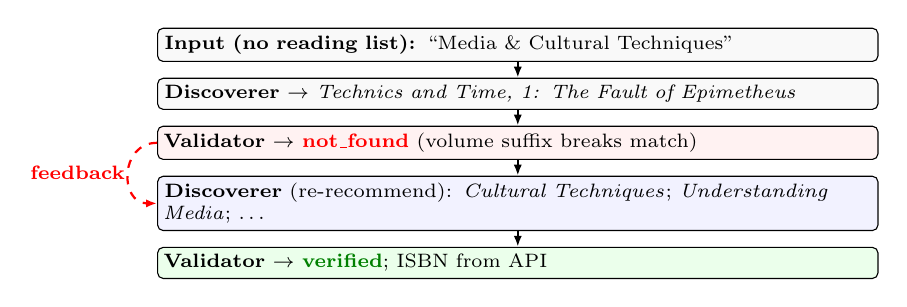
\begin{tikzpicture}[
    font=\scriptsize,
    box/.style={draw, rounded corners=2pt, align=left, inner sep=2.5pt,
                text width=0.74\columnwidth, fill=gray!5, font=\scriptsize},
    lbl/.style={font=\scriptsize\bfseries, inner sep=1pt},
    arr/.style={-{Latex[length=1.4mm]}, thick},
]
\node[box] (input) {\textbf{Input (no reading list):} ``Media \& Cultural Techniques''};
\node[box, below=2mm of input] (rec1) {\textbf{Discoverer} $\rightarrow$
    \textit{Technics and Time, 1: The Fault of Epimetheus}};
\node[box, below=2mm of rec1, fill=red!5] (val1) {\textbf{Validator} $\rightarrow$
    \textcolor{red}{\textbf{not\_found}} (volume suffix breaks match)};
\node[box, below=2mm of val1, fill=blue!5] (rec2) {\textbf{Discoverer} (re-recommend):
    \textit{Cultural Techniques}; \textit{Understanding Media}; \dots};
\node[box, below=2mm of rec2, fill=green!8] (val2) {\textbf{Validator} $\rightarrow$
    \textcolor{green!50!black}{\textbf{verified}}; ISBN from API};
\draw[arr] (input) -- (rec1);
\draw[arr] (rec1) -- (val1);
\draw[arr] (val1) -- (rec2);
\draw[arr] (rec2) -- (val2);
\draw[arr, red, dashed] (val1.west) to[out=180, in=180, looseness=1.6]
    node[left, lbl, text=red]{feedback} (rec2.west);
\end{tikzpicture}
\caption{An example execution trace of the feedback loop. For a course with no
reading list, the Discoverer recommends a reference that fails verification (its
volume suffix breaks exact matching); the failure signal is routed back, and the
re-recommended alternatives are verified successfully.}
\label{fig:trace}
\end{figure}

\textit{Verification-driven feedback loop.} On top of this linear pipeline, we
add a conditional edge from the Validator to the Discoverer, forming a
self-correcting closed loop (Fig.~\ref{fig:trace}). When a book recommended by
the Discoverer (\texttt{[AI-recommended]} and verified as
\texttt{\seqsplit{not\_found}}/\texttt{\seqsplit{ncl\_not\_found}}, excluding
transient failures due to quota exhaustion) fails
verification, a routing function redirects control flow back to the Discoverer,
which re-recommends an alternative given the knowledge that the previous
recommendation was verified as nonexistent; the alternative is re-verified
until success or an iteration cap (set to 2). The loop acts only on
AI-recommended books, not on those extracted by the Parser from the
syllabus; for the latter, a verification failure may simply mean the syllabus
did list the book but the source has not cataloged it, so replacement is
unwarranted. Failed old records are not deleted but marked with a
\texttt{\seqsplit{superseded\_by\_iteration}} field for traceability; downstream queries
exclude superseded records. The iteration counter is incremented by the
Validator and only read by the routing function, ensuring the loop terminates.

\subsection{Evaluation Design}
\textbf{Metric definitions.} Our two core metrics are defined as follows.
\textit{Generation correctness} measures whether a generated bibliographic
entry should appear in the given course: for books listed in the syllabus,
whether it correctly corresponds to a book actually present in the syllabus
text; for AI-recommended books, whether it is a reasonable reference that is
both topically relevant and real. \textit{Hallucination rate} measures whether
a generated entry (title/ISBN) points to a real book: an entry that cannot be
mapped to any real authoritative record (including a fabricated title, or a
real author paired with a nonexistent title) is counted as a hallucination.
Both metrics are judged manually as binary yes/no; annotation uses stratified
sampling (prioritizing cases where the conditions disagree or the pre-screen
flags a suspected issue), supported by external bibliographic API lookups.
Correctness and hallucination are independent dimensions: an entry may be real
yet not belong to the course, and vice versa. These two metrics
evaluate the generation side (Section IV.A); the verifier's pairing quality is
measured separately by the mis-pairing rate (Experiment 2).

\textbf{Experiment 1 (architecture comparison).} To assess the effect of
``granting a verification tool'' on generation-side reliability, we design two
generation-side baselines that receive the same input and use the same base
prompt, differing only in whether they can verify. All conditions use the same underlying model (GPT-5.5 via an OpenAI-compatible
API, a reasoning model run at its required temperature of 1). The base prompt
asks the model to extract listed books and (when the syllabus lists none)
recommend 3--5 references in a single pass, producing structured JSON.
\textit{Both baselines retain the system's original anti-hallucination
constraints} (ISBN only from
the source text, uncertain fields left blank), ensuring each baseline performs
at its best and avoiding a deliberately weakened (straw-man) control that would
exaggerate the system's advantage. Condition A (pure LLM) provides no tools,
measuring the upper bound of pure generation-side reliability; Condition B
provides a single \texttt{search\_book(title, authors)} tool (backed by the
same bibliographic sources the Validator uses), with the model deciding
autonomously in a multi-round loop whether to call it and whether to trust the
results, measuring the effect of granting a tool used at the model's
discretion. Their difference reflects the value of granting a verification
tool. In addition, our system (denoted C) enforces external verification on
every book, with the ISBN determined by the API; its design is described in
Section III.B and its verifier's pairing reliability analyzed in Experiment 2;
because C additionally undergoes authoritative-record pairing and its output
object differs from A/B, we do not place it alongside the generation-side
baselines in the correctness comparison.

\textbf{Experiment 2 (verifier reliability).} We analyze pairing errors among
Chinese books that the Validator reported as \emph{successfully} verified (i.e.,
the mis-match rate is conditional on verification success, a different population
from the failure-cause diagnosis of Experiment 4). We stratify into short titles
($\leq 4$ characters) and general titles and sample 60 of each; because the
strata are sampled 1:1 by design, we report the two stratum rates separately,
and, to obtain a corpus-level estimate, additionally weight them by the true
composition of the 1{,}468 successfully verified Chinese books (short titles
19.3\%, general 80.7\%). We also ablate the SRU candidate-window size
(maximumRecords) between 5 and 20.

\textbf{Experiment 3 (feedback loop).} We evaluate the loop's benefit on the
verification success rate of AI-recommended books. To isolate the randomness of
LLM generation, the ``no-loop'' and ``with-loop'' arms share the same initial
recommendation: a single recommendation and verification pass serves as the
common starting point, the no-loop arm takes this first-pass result, and the
with-loop arm continues from the same state to trigger re-recommendation. It
covers 50 courses requiring AI recommendation.

\textbf{Experiment 4 (failure-cause diagnosis).} We classify
verification-failed (not\_found / ncl\_not\_found) books by cause into three
types: \textbf{(T1) recovered-after-fix}, retrieved after title normalization
(stripping volume suffixes, subtitles, traditional--simplified differences)
with author-matched queries; \textbf{(T2) unresolved query defect}, still
missed after the fix, but a loose query finds a highly similar title (i.e., the
book exists but exact matching still fails); and \textbf{(T3) coverage gap},
where even a loose query finds no similar result (i.e., the source has not cataloged it). T1
and T2 together are termed ``query-related'' failures (resolvable by improving
query logic), while T3 requires source expansion. English books use the full
set (49), and Chinese books a random sample ($n=100$, population 481, fixed
random seed). Book existence is probed with loose queries against the National
Central Library (NCL) for Chinese and Google Books/LOC for English; because
coverage of any single source is imperfect, the reported coverage gap is an
upper-bound estimate.

\textbf{Annotation and statistics.} Manual annotation uses binary yes/no
judgments. To assess reliability, a second annotator independently labeled all
70 architecture-comparison rows against the same rubric (judging correctness by
consulting the original syllabus text rather than title--topic similarity).
Inter-annotator agreement is 98.5\% overall (98.6\% for correctness, 98.5\% for
hallucination); because the labels are highly imbalanced (the positive class
dominates), which renders Cohen's $\kappa$ uninformative, we report Gwet's
AC1${}=0.985$ (almost-perfect agreement). Because of stratified sampling and
limited sample size, the reported proportions are observational; 95\% confidence
intervals are computed with the Wilson interval. All experiments count by
citation, including cross-course repeated citations.

% ============================================================
\section{Results and Discussion}

\subsection{Architecture Comparison: Hallucination Is Not the Bottleneck}
We compare the two generation-side baselines (A, B), which output only titles,
against our full system (C), whose end-to-end output additionally passes through
the verifier's authoritative-record pairing. For A and B, correctness judges
only the generated title; for C, it judges the end-to-end result, so a title
that is generated correctly but paired to an irrelevant authoritative record
counts as incorrect (the acquisition-usable output is the paired record). The
three are therefore not measuring an identical object, and we make this explicit
rather than omit C, because C's number is central to our argument.

% 表 1：生成端 baseline + 系統，置於 IV.A
\begin{table}[t]
\caption{Correctness and Hallucination Rate of Generation-Side Baselines (A, B)
and the Full System (C) ($n=70$; 95\% CI by Wilson Interval)}
\label{tab:baseline}
\centering
\small
\setlength{\tabcolsep}{4pt}
\begin{tabular}{lccc}
\toprule
Metric & A (pure LLM) & B (LLM+tool) & C (system) \\
\midrule
Correctness & 98.6\% & 100\% & 80.0\% \\
            & (69/70) & (70/70) & (28/35) \\
\quad 95\% CI & 92.3--99.7\% & 94.8--100\% & 64.1--90.0\% \\
Hallucination & 0\% & 1.4\% & --- \\
\quad 95\% CI & 0--5.2\% & 0.3--7.7\% & --- \\
\bottomrule
\end{tabular}

\vspace{2pt}
{\scriptsize A/B correctness judges the generated title; C judges the end-to-end
result (generation + verifier pairing). C's $n{=}35$ counts only books that
reached the verifier's pairing stage. C's ISBN is API-determined, so C has no
hallucination by construction.}
\end{table}

Table~\ref{tab:baseline} reports the results. The generation side (A, B) shows
uniformly high correctness (98.6--100\%) and uniformly low hallucination rates
(0--1.4\%). Even in Condition A, with no external tools, the hallucination rate
is 0\%, indicating that, under anti-hallucination prompt constraints, LLMs are
already quite reliable at generating real bibliographies. Condition B's sole
hallucination case is not ``fabrication from nothing'' but ``mislabeling'': the
model paired a real author with an incorrectly remembered title. Held with high
confidence and internally plausible, such errors evade prompt constraints and
existence checks alike, and can be caught only through external
title--author cross-checking.

One might object that this low rate merely reflects an easy task: entries
extracted from a listed syllabus are transcribed, not generated. Splitting the
70 entries by provenance refutes this. The \emph{AI-recommended} subset, 40
entries whose course listed no readings, so the model generated from the
description alone, shows a 0\% hallucination rate (0/40; Wilson 95\% CI
0--8.8\%), whereas the single hallucination falls in the \emph{extracted} subset.
The low rate is thus not an artifact of task simplicity; the small $n$ warrants
caution, but the direction counters the objection.

Critically, our full system (C) scores markedly \emph{lower} (80.0\%) than its
own generation side (A/B). Since C's titles originate from the same reliable
generation but then pass through the verifier's authoritative-record pairing,
this 18--20 point drop is attributable entirely to verifier mis-pairing: all
seven incorrect cases involve a book paired to an irrelevant authoritative
record (e.g., a scripture title paired to a stage-drama performance record), not
an honest ``not found,'' consistent with this sample being conditioned on
verification success, whereas coverage gaps (Section IV.C) dominate the
complementary population of verification failures. This is direct evidence,
within a single experiment, that the bottleneck is not generation but the
verification stage. We analyze this failure in the next subsection.

\subsection{Verification Is Needed, but the Verification Stage Is the
Bottleneck: A Three-Layer Failure Structure}
Given the reliable generation side, where do errors come from? The verification
stage remains \textit{necessary}: the titles A/B produce lack ISBNs and cannot
be traced, and only after external verification yields a traceable authoritative
record does the output become actionable. The question is not ``whether to
verify'' but its reliability. Combining the four experiments, verification
failures resolve into a three-layer structure:

\begin{enumerate}
\item \textbf{LLM hallucination (rare).} A/B hallucination rate 0--1.4\%; not
the primary problem.
\item \textbf{Verifier mis-pairing (a correctable pairing defect).} The
verifier finds a book but pairs it to an irrelevant authoritative record; for
example, a scripture title paired to a stage-drama performance record. Experiment
2 quantifies this among verified Chinese books: short titles ($\leq 4$ characters)
mis-pair at 66.7\% ($n=60$), far exceeding general titles at 25.0\% ($n=60$).
Weighting the two strata by the true corpus composition (short titles 19.3\%,
general 80.7\% of the 1{,}468 verified Chinese books) yields a corpus-level
mis-pairing rate of 33.1\% (versus 45.8\% under the 1:1 design weighting)---%
coincidentally close to, but a distinct quantity from, the 33.0\%
normalization-recovery rate reported below. This
confirms short titles easily mis-pair to irrelevant records in bibliographic
databases. Such failures are improvable
through query
normalization. Experiment 4 shows that, in an offline replay of the failed
Chinese entries, 33.0\% are directly recovered after our title normalization
(stripping volume suffixes, subtitles, traditional--simplified differences). A
representative case is
\textit{Technics and Time, 1}: its trailing volume suffix (``, 1'') causes
exact phrase matching to fail, and after the fix its authoritative record is
retrieved (ISBN 9780804730419).
\item \textbf{Coverage gap (requiring source expansion).} Many genuinely
existing books are simply absent from the queried library-cataloging sources,
most acutely English academic works and specific editions. Experiment 4 shows
this accounts for 61.2\% of English failures and 50.0\% of Chinese
(upper-bound estimate). Such failures cannot be solved by the pairing algorithm
and require integrating more sources; the system correctly keeps such books as
``not found'' rather than mis-pairing them to raise the hit rate.
\end{enumerate}

The genuine bottleneck is thus pairing quality (fixable by engineering) and
source coverage (requiring more resources), not generation-side hallucination.
Widening the candidate window from 5 to 20 improves resolvable cases by only 11.8
percentage points (64.7\% still unresolved), confirming the problem is not
candidate selection but these two deeper layers.

\subsection{Failure-Cause Diagnosis}
% 表 2：失敗成因診斷，置於 IV.C
\begin{table}[t]
\caption{Cause Classification of First-Pass Verification Failures}
\label{tab:cause}
\centering
\small
\setlength{\tabcolsep}{4pt}
\begin{tabular}{lcc}
\toprule
Failure cause & English (49) & Chinese (100) \\
\midrule
T1 recovered-after-fix     & 12.2\% (6)  & 33.0\% (33) \\
T2 unresolved query defect & 26.5\% (13) & 17.0\% (17) \\
T3 coverage gap            & 61.2\% (30) & 50.0\% (50) \\
\textbf{Query-related (T1+T2)} & \textbf{38.8\% (19)} & \textbf{50.0\% (50)} \\
\bottomrule
\end{tabular}
\end{table}

Table~\ref{tab:cause} reports the cause classification. The structures differ
markedly: English failures are dominated by coverage gaps (61.2\%), whereas half
of Chinese failures (50.0\%) are query-related. The design implication is that
query normalization has the highest marginal benefit for Chinese, while English
requires expanding source coverage. The Chinese coverage gap (50.0\%) is an
upper-bound estimate, counted by citation (including cross-course repeats).

\subsection{Feedback Loop: The Benefit Ceiling Depends on Failure Cause}
The loop acts only on books recommended by the Discoverer. Across 50 courses
and 249 AI-recommended books, the first-pass verification success rate already
reaches 99.2\% (only 2 failures); the loop handles both, but because the room
for improvement is small, the absolute gain is only 0.8 percentage points. The
two failures have different causes: one a query defect (a volume suffix), the
other a coverage gap. This reveals the loop's fundamental limit: when failure
stems from the model recommending incorrectly, re-recommendation fixes it; when
it stems from a genuinely existing book absent from the sources, re-recommending
merely circumvents the verifier's blind spot. The loop's benefit ceiling is thus
bounded by the structure of failure causes.

\subsection{Implications for Multi-Agent System Design}
Since the LLM generation side is already highly accurate, a multi-agent
architecture's value lies not in raising accuracy but in
\textit{auditability}, meaning every item is traceable to an external
authoritative record (ISBN API-determined, not model-generated), and
\textit{error-catching}: a dedicated, enforced verification agent catches
detail-level ``mislabeling'' that prompt constraints cannot prevent.

A concrete case makes the auditability payoff tangible. For the short title
\textit{Yuball zhinan} (Badminton Guide), the verifier returned an authoritative
record for \textit{Illustrated Swimming Guide}, a different sport, mis-paired on
a shared trailing word. Because the pipeline persists the original citation
alongside the paired record, the human-review node surfaces this title--author
mismatch and flags it for correction; in a generate-only system with no retained
provenance, the wrong record would flow silently into the purchase list.
Auditability here is not an abstract virtue but the mechanism that makes such an
error \emph{catchable at all}.

On Condition B (model-autonomous tool use) versus C (enforced verification): the
two perform comparably here, as B invokes the tool at a high rate. So ``enforced
verification is superior'' is an \textit{architecture-level argument, not an
experimentally confirmed conclusion}: B offers no procedural guarantee, whereas C
ensures 100\% coverage and auditability; its advantage under adversarial or
large-scale conditions awaits future work.

\subsection{Implications for Educational Technology}
This is also a rare \emph{deployed} educational-technology case, exercised over
an institution's full semester (7{,}354 courses) rather than a curated benchmark,
and portable: the agents rely only on standard protocols (SRU) and public
catalog APIs, so adapting to another university requires little beyond swapping
the holdings endpoint, positioning LLM multi-agent verification as reusable
educational infrastructure, not a one-off script.

\subsection{Limitations}
Four limitations apply. The data is one institution's single semester, limiting
external validity. The annotation sample is limited (70 for the architecture
comparison, 50 courses for the loop, 149 for the diagnosis); despite
almost-perfect inter-annotator agreement (AC1${}=0.985$), proportions remain
observational rather than significant (95\% CIs tabulated). Chinese existence
probing queries the NCL union catalog, falling back to Google Books (which
under-covers traditional-Chinese books), so the Chinese coverage-gap figure
(50.0\%) is an upper bound; moreover, because the T2/T3 boundary is decided by a
loose external lookup, the exact split may shift by a few entries as source
indices change (our reported figures are reproducible from the released
classification log). Finally, the feedback-loop evaluation rests on only
two triggering failures, so its benefit estimate is illustrative rather than
conclusive.

% ============================================================
\section{Conclusion and Future Work}

We presented a six-agent LLM system (plus a human-review node) for
course-syllabus analysis and library acquisition, augmented with a
Validator$\rightarrow$Discoverer feedback loop. Across four experiments, the
bottleneck proved to be verification, namely record mis-pairing and source
coverage gaps, rather than generation-side hallucination (0--1.4\%); a
multi-agent
architecture's value here thus lies not in preventing hallucination but in
auditability and detail-level error-catching. Two directions follow: expanding
source coverage (most failed books appear in commercial trade-bibliography
sources), and cross-institutional, larger datasets to test enforced versus
model-autonomous verification.

% ============================================================
\enlargethispage{2\baselineskip}
{\fontsize{9}{10}\selectfont
\begin{thebibliography}{00}
\bibitem{ReAct} S. Yao et al., ``ReAct: Synergizing reasoning and acting in language models,'' arXiv:2210.03629, 2023.
\bibitem{RAG} P. Lewis et al., ``Retrieval-augmented generation for knowledge-intensive NLP tasks,'' in \textit{NeurIPS}, vol.\ 33, pp.\ 9459--9474, 2020.
\bibitem{FactScore} S. Min et al., ``FActScore: Fine-grained atomic evaluation of factual precision in long form text generation,'' in \textit{Proc.\ EMNLP}, Dec.\ 2023, pp.\ 12076--12100.
\bibitem{RAGAS} S. Es, J. James, L. Espinosa-Anke, and S. Schockaert, ``RAGAS: Automated evaluation of retrieval augmented generation,'' in \textit{Proc.\ EACL: System Demonstrations}, Mar.\ 2024, pp.\ 150--158.
\bibitem{LLMJudge} L. Zheng et al., ``Judging LLM-as-a-judge with MT-Bench and Chatbot Arena,'' in \textit{NeurIPS}, vol.\ 36, 2023.
\bibitem{SIE} J. Dagdelen, A. Dunn, et al., ``Structured information extraction from scientific text with large language models,'' \textit{Nature Communications}, vol.\ 15, art.\ 1418, 2024, doi: 10.1038/s41467-024-45563-x.
\bibitem{DSS} M. Hemili, A. Laouar, and S. B. Eom, ``A decision support system for managing demand-driven collection development in university digital libraries,'' \textit{Int. J. of Information Systems and Social Change}, vol.\ 10, no.\ 4, pp.\ 57--74, 2019.
\end{thebibliography}}

\end{document}
